  \documentclass[a4]{beamer}
\usepackage{amssymb}
\usepackage{graphicx}
\usepackage{subfigure}
\usepackage{newlfont}
\usepackage{amsmath,amsthm,amsfonts}
%\usepackage{beamerthemesplit}
\usepackage{pgf,pgfarrows,pgfnodes,pgfautomata,pgfheaps,pgfshade}
\usepackage{mathptmx} % Font Family
\usepackage{helvet} % Font Family
\usepackage{color}
\mode<presentation> {
\usetheme{Default} % was Frankfurt
\useinnertheme{rounded}
\useoutertheme{infolines}
\usefonttheme{serif}
%\usecolortheme{wolverine}
% \usecolortheme{rose}
\usefonttheme{structurebold}
}
\setbeamercovered{dynamic}
\title[MA4603]{Science Mathematics 3 \\ {\normalsize MA4603 Lecture 3B/4A}}
\author[Kevin O'Brien]{Kevin O'Brien \\ {\scriptsize kevin.obrien@ul.ie}}
\date{Spring 2013}
\institute[Maths \& Stats]{Dept. of Mathematics \& Statistics, \\ University \textit{of} Limerick}
\renewcommand{\arraystretch}{1.5}
%------------------------------------------------------------------------%
\begin{document}
	
	\begin{frame}
		\titlepage
	\end{frame}

%------------------------------------------------------------%
\begin{frame}

\frametitle{Introduction to the Normal Distribution}
\begin{itemize}
\item
Recall the experiment whereby a die was rolled 100 times, and the sum of the 100 values was recorded.
\item
This experiment was repeated a very large number of times (e.g. 100,000 times ) in a simulation study.
\item
A histogram was drawn to depict the distribution of outcomes of this experiment.
\item Recall that we agreed that ``bell-shaped" was a good description of the histogram.

\end{itemize}
\end{frame}


\frame{
\frametitle{Normal Distribution}

\begin{center}
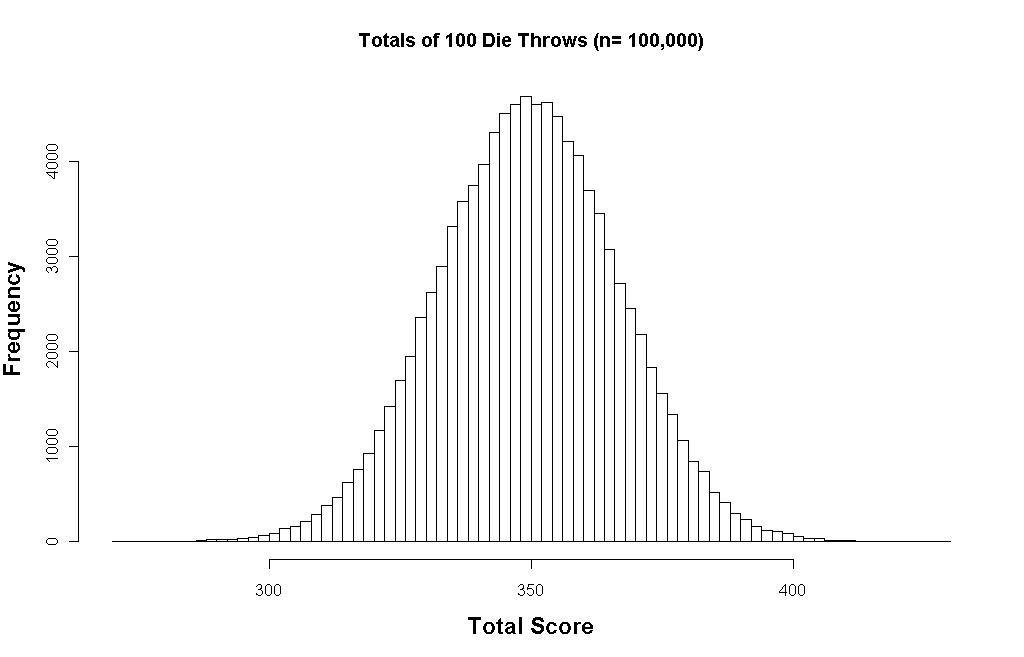
\includegraphics[scale=0.30]{images/3aDieHist3}
\end{center}

}
%----------------------------------------------------------------------%

\frame{
\frametitle{Normal Distribution}
\begin{itemize}
\item The normal distribution is perhaps the most widely used distribution for a random variable.
\item Normal distributions have the same general shape: the bell curve.
\item The distributions are \textbf{symmetric} with values concentrated more in the middle than in the tails.
%\item Examples of normal distributions are shown below. Notice that they differ in how spread out they are. The area under each curve is the same.
\item \alert{Important} The height of a normal distribution can be defined mathematically in terms of two fundamental parameters: the normal mean ($\mu$) and the normal
    standard deviation ($\sigma$).
\item A normally distributed random variable X is denoted $ X \sim \mbox{N} (\mu, \sigma^2)$ (note that we use the variance term here)
    \item The mean ($\mu$) and standard deviation ($\sigma$) are vital for calculating probabilities.
\end{itemize}
}
%------------------------------------------------------------------------%
\frame{
\frametitle{The Normal Distribution}
The \textbf{\emph{probability density function}} of the normal distribution is given as
\[ f(x) = \frac{1}{\sqrt{2\pi\sigma^2}} e^{ -\frac{(x-\mu)^2}{2\sigma^2} } \]

Integrating this formula would allow us to compute probabilities.
However, it is not required to use this formula.
}
%------------------------------------------------------------------%
\frame{
\frametitle{Normal Distribution}
\vspace{-0.25cm}
\begin{center}
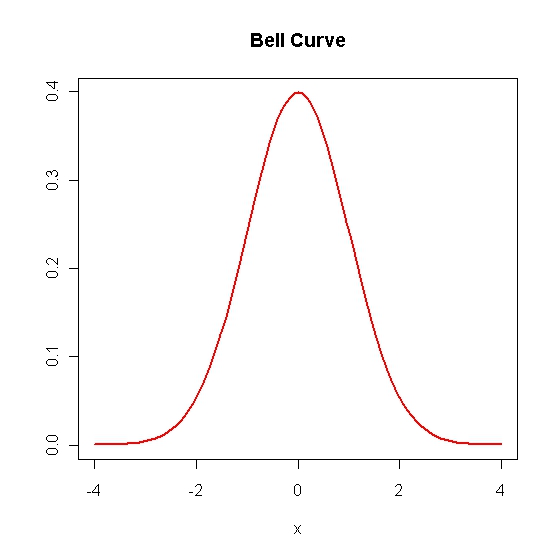
\includegraphics[scale=0.450]{images/5ABellCurve}
\end{center}

}

%------------------------------------------------------------------------%
\section{Using the Murdoch Barnes Tables 3}
\frame{
\frametitle{Using Murdoch Barnes Tables 3}
\begin{itemize}
\item For some value $z_o$, between 0 and 4, the Murdoch Barnes tables set 3 tabulate $P(Z \geq z_o)$
\item Ideally $z_o$ would be specified to 2 decimal places. If it is not, round to the closest value.
\item We call the third digit (i.e. the digit in the second decimal place) the ``second precision".
\end{itemize}
}

%------------------------------------------------------------------------%
\frame{
\frametitle{Using Murdoch Barnes Tables 3}
\begin{itemize}
\item To compute the relevant probability we express $z_o$ as the sum of $z_o$ without the second precision, and the second precision.(For example $1.28 = 1.2 + 0.08$.)
\item Select the row that corresponds to $z_o$ without the second precision (e.g. 1.2).
\item Select the column that corresponds to the second precision(e.g. 0.08).
\item The value that contained on the intersection is $P(Z \geq z_o)$
\end{itemize}
}

%------------------------------------------------------------------------%
\frame{
\begin{table}[ht]
\frametitle{Find $ P(Z \geq 1.28)$}
\vspace{-1.5cm}
%\caption{Standard Normal Distribution } % title of Table
\centering % used for centering table
\begin{tabular}{|c|| c c c c c c|} % centered columns (4 columns)
\hline %inserts double horizontal lines
& \ldots & \ldots & 0.006 &0.07&0.08&0.09 \\
%heading
\hline \hline% inserts single horizontal line
\ldots & \ldots & \ldots &\ldots& \ldots &\ldots&\dots \\ % inserting body of the table
1.0 & \ldots & \ldots &0.1446& 0.1423 &0.1401&0.1379 \\ % inserting body of the table
1.1 & \ldots & \ldots&0.1230& 0.1210 &0.1190&0.1170 \\ % inserting body of the table
1.2 & \ldots & \ldots&0.1038 & 0.1020 &\alert{0.1003}&0.0985\\
1.3 & \ldots & \ldots &0.0869& 0.0853 &0.0838&0.0823 \\ % inserting body of the table
\ldots & \ldots &\ldots&\ldots & \ldots &\ldots&\ldots\\
\hline %inserts single line
\end{tabular}
%\label{table:nonlin} % is used to refer this table in the text
\end{table}
}

%------------------------------------------------------------------------%
\frame{
\frametitle{Using Murdoch Barnes tables 3}
\begin{itemize}
\item Find $ P(Z \geq 0.60)$
\item Find $ P(Z \geq 1.64)$
\item Find $ P(Z \geq 1.65)$
\item Estimate $P( Z \geq 1.645)$
\end{itemize}
}

%------------------------------------------------------------------------%
\frame{
\begin{table}[ht]
\frametitle{Find $ P(Z \geq 0.60)$}
\vspace{-1.5cm}
%\caption{Standard Normal Distribution } % title of Table
\centering % used for centering table
\begin{tabular}{|c|| c c c c c c|} % centered columns (4 columns)
\hline %inserts double horizontal lines
& 0.00 & 0.01 & 0.02 &0.03&\ldots&\ldots \\
%heading
\hline \hline% inserts single horizontal line \hline
\ldots & \ldots &\ldots &\ldots& \ldots &\ldots&\ldots \\ % inserting body of the table
0.4 & 0.3446 & 0.3409&0.3372 & 0.3336 &\ldots&\ldots\\
0.5 & 0.3085 & 0.3050 &0.3015& 0.2981 &\ldots&\dots \\ % inserting body of the table
0.6 & \alert{0.2743} & 0.2709&0.2676 & 0.2643 &\ldots&\ldots\\
0.7 & 0.2420 & 0.2389 &0.2358& 0.2327 &\ldots&\dots \\ % inserting body of the table
\ldots & \ldots &\ldots &\ldots& \ldots &\ldots&\ldots \\ % inserting body of the table
\hline %inserts single line
\end{tabular}
%\label{table:nonlin} % is used to refer this table in the text
\end{table}
}

%------------------------------------------------------------------------%
\frame{
\begin{table}[ht]
\frametitle{Find $ P(Z \geq 1.64)$ and $ P(Z \geq 1.65)$}
\vspace{-1.5cm}
%\caption{Standard Normal Distribution } % title of Table
\centering % used for centering table
\begin{tabular}{|c|| c c c c c c|} % centered columns (4 columns)
\hline %inserts double horizontal lines
& \ldots & \ldots & 0.04 & 0.05 &0.06&0.07 \\
%heading
\hline \hline% inserts single horizontal line
\ldots & \ldots &\ldots &\ldots& \ldots &\ldots&\ldots \\ %Checked
1.5 & \ldots & 0.0630&0.0618& 0.0606 &0.0594&\dots \\ % inserting body of the table
1.6 & \ldots &0.0516& \alert{0.0505} & \alert{0.0495} &0.0485&\ldots\\
1.7 & \ldots &0.0418 &0.0409& 0.0401 &0.0392&\dots \\ % inserting body of the table
\ldots & \ldots &\ldots &\ldots& \ldots &\ldots&\ldots \\ %Checked
\hline %inserts single line
\end{tabular}
%\label{table:nonlin} % is used to refer this table in the text
\end{table}
}

%------------------------------------------------------------------------%
\frame{
\frametitle{Using Murdoch Barnes tables 3}
\begin{itemize}
\item $ P(Z \geq 1.64) = 0.505$
\item $ P(Z \geq 1.65) = 0.495$ \bigskip
\item $ P(Z \geq 1.645)$ is approximately the average value of $ P(Z \geq 1.64)$ and $ P(Z \geq 1.65)$.
\item $ P(Z \geq 1.645)$ = (0.0495 + 0.0505)/2 = 0.0500. ( i.e. $5\%$ )
\end{itemize}
}
%------------------------------------------------------------------%
\frame{
\frametitle{Exact Probability}
\large
\alert{Remarks:} This is for continuous distributions only.
\begin{itemize}
\item The probability that a continuous random variable will take an exact value is infinitely small.
We will usually treat it as if it was zero.
\item
When we write probabilities for continuous random variables in mathematical notation, we often retain the equality component (i.e. the "...or equal to..").\\
For example, we would write expressions $P(X \leq 2)$ or $P(X \geq 5)$.
\item
Because the probability of an exact value is almost zero, these two expression are equivalent to $P(X < 2)$
or $P(X > 5)$. \item The complement of $P(X \geq k)$ can be written as $P(X \leq k)$.
\end{itemize}
}


%------------------------------------------------------------------%
\frame{
\frametitle{Complement and Symmetry Rules}

Any normal distribution problem can be solved with some combination of the following rules.
\begin{itemize} \item \textbf{Complement rule} \item Common to all continuous random variables
\[P(Z \geq k) = 1 - P(Z \leq k) \]
Similarly
\[P(X \geq k) = 1 - P(X \leq k) \]
\end{itemize}

\[P(Z \leq 1.28) = 1 - P(Z \geq 1.28)  = 1-0.1003 = 0.8997\]
}

%------------------------------------------------------------------%
\frame{
\frametitle{Complement and Symmetry Rules}
\begin{itemize}
\item \textbf{Symmetry rule}
\item
This rule is based on the property of symmetry mentioned previously.
\item
Only the probabilities corresponding to values between 0 and 4 are tabulated in Murdoch Barnes.
\item
If we have a negative value of k, we can use the symmetry rule.
\end{itemize}
\[P(Z \leq -k) = P(Z \geq k) \]
by extension, we can say
\[P(Z \geq -k) = P(Z \leq k) \]
}
%------------------------------------------------------------------%
\frame{
\frametitle{Z Scores: Example 1 }
Find $P(Z \geq -1.28)$\\
\textbf{Solution}\\
\begin{itemize}
\item Using the symmetry rule
\[P(Z \geq -1.28) = P(Z \leq 1.28) \]
\item Using the complement rule
\[P(Z \geq -1.28) = 1 - P(Z \geq 1.28) \]
\[P(Z \geq -1.28) = 1 - 0.1003 = 0.8997 \]
\end{itemize}
}
%------------------------------------------------------------------%
\frame{
\frametitle{Z Scores: Example 2 }
Find the probability of a ``z" random variable being between -1.8 and 1.96?
i.e. Compute $P(-1.8 \leq Z \leq 1.96)$\\
Solution
\begin{itemize}
\item Consider the complement event of being in this interval: a combination of being too low or too high.
\item
The probability of being too low for this interval is $P(Z \leq -1.80) = 0.0359$ (check)
\item
The probability of being too high for this interval is $P(Z \geq 1.96) = 0.0250$ (check)
\item
Therefore the probability of being \textbf{outside} the interval is 0.0359 + 0.0250 = 0.0609.
\item
Therefore the probability of being \textbf{inside} the interval is 1- 0.0609 = 0.9391
$P(-1.8 \leq Z \leq 1.96) = 0.9391$
\end{itemize}
}





%--------------------------------------------------------------
\begin{frame}
\frametitle{Application : Example }
The mean time spent waiting by customers before their queries are dealt with at an information centre is 10 minutes.\\ \smallskip
The waiting time is normally distributed with a standard deviation of 3 minutes.
\begin{itemize}
\item [i)] What percentage of customers will be waiting longer than 15 minutes

\item [ii)] $90\%$ of customers will be dealt with in at most 12 minutes. Is this statement true or false?
Justify your answer.

\item [iii)] What percentage of customers will wait between 7 and 13 minutes before their query is dealt with?
\end{itemize}
\end{frame}
%---------------------------------------------%
\begin{frame}
\frametitle{Solutions}

Let x be the normal random variable describing waiting times\\
$P(X \geq 15) =?$ \\
\bigskip
     First , we find the z-value that corresponds to x = 15  (remember $\mu=10$ and $\sigma=3$  )\\
\[ z_o = { x_o - \mu \over \sigma }  = { 15 - 10 \over 3 } = 1.666 \]
\begin{itemize}
\item We will use $z_o =1.67$
\item Therefore we can say $P(X \geq 15 ) = P(Z \geq 1.67)$
\item The Murdoch Barnes tables are tabulated to give $P(Z \geq z_o)$ for some value $ z_o$ .
\item We can evaluate $P(Z \geq 1.67)$  as 0.0475.
\item Necessarily $P(X \geq 15) = 0.0475$.
\end{itemize}
\end{frame}

%---------------------------------------------%
\begin{frame}
\frametitle{Solutions}
\begin{itemize}
\item "$90\%$ of customers will be dealt with in at most 12 minutes."
\item To answer this question, we need to know  $P(X\leq 12)$
\item First , we find the z-value that corresponds to x = 12  (remember $\mu=10$ and $\sigma=3$ )
\end{itemize}
\[ z_o = { x_o - \mu \over \sigma }  = { 12 - 10 \over 3 } = 0.666 \]

\end{frame}

%---------------------------------------------%
\begin{frame}
\frametitle{Solutions}
\begin{itemize}
\item We will use $z_o =0.67$ (although 0.66 would be fine too) 
\item Therefore we can say $P(X \geq 12 ) = P(Z \geq 0.67)  = 0.2514$
\item Necessarily  $P(X \leq 12 ) = P(Z \leq 0.67) = 0.7486$
\item $74.86\%$ of customers will be dealt with in at most 12 minutes.
\item The statement that $90\%$ will be dealt with in at most 12 minutes is false.
\end{itemize}
\end{frame}
%---------------------------------------------%
\begin{frame}
\frametitle{Solutions}
What percentage will wait between 7 and 13 minutes ?\\

\[P(7 \leq X \leq 13)   = ?\]

\textbf{Solution:}
\begin{itemize}
	\item Compute the probability of being too low, and the probability of being too high for the interval.\item The probability of being inside the interval is the complement of the combination of these events.
\end{itemize}

\end{frame}
%---------------------------------------------%
\begin{frame}
\frametitle{Solutions}
\textbf{Too high:}\\
$P(X \geq 13) = ?$
\[ z_o  = {13 - 10  \over 3} = 1\]
\smallskip
From tables, $P(Z \geq 1) = 0.1587$. Therefore $P(X \geq 13) = 0.1587$\\ \bigskip
\textbf{Too low:}\\
$P(X \leq 7) = ?$
\[ z_o  = {7 - 10  \over 3} = -1\]
By symmetry, and using tables, $P(X \leq 7) = P(Z \leq -1)= 0.1587$\\ \bigskip
\end{frame}
%---------------------------------------------%
\begin{frame}
\frametitle{Solutions}

\[P(7 \leq X \leq 13)  = 1 - [ P(X \leq 7)  + P(X \geq 13) ] \]

\[P(7 \leq X \leq 13)  =  1 - [0.1587+0.1587] = 0.6826\]

\end{frame}

%-----------------------------------------------------%
\begin{frame}
\frametitle{Normal Distribution : Solving problems}
Recap:
\begin{itemize}
\item We must know the normal mean $\mu$ and the normal standard deviation $\sigma$.
\item The normal random variable is $X \sim \mbox{N} ( \mu , \sigma^2)$.\smallskip
\item (If we don't, we usually have to determine them, given the information in the question.)\smallskip
\item The standard normal random variable is $Z\sim \mbox{N} ( 0 , 1^2)$.\smallskip
\item The standard normal distribution is well described in Murdoch Barnes Table 3, which tabulates $P(Z \geq z_o)$ for a range of $Z$ values.
\end{itemize}
\end{frame}
%-----------------------------------------------------%
\begin{frame}
\frametitle{Normal Distribution : Solving problems}
\begin{itemize}
\item For the given value $x_o$ from the variable $X$, we compute the corresponding z-score $z_o$.
\[ z_o = { x_o - \mu \over \sigma} \]
\item When $z_o$ corresponds to $x_o$, the following identity applies:
\[  P(X \geq x_o )= P(Z \geq z_o ) \]
\item Alternatively $ P(X \leq x_o )= P(Z \leq z_o ) $
\end{itemize}
\end{frame}
%-----------------------------------------------------%
\begin{frame}
\frametitle{Normal Distribution : Solving problems}
\begin{itemize}
\item \textbf{Complement Rule}: \[ P(Z \leq k) = 1-P(Z \geq k) \] for some value $k$
\item Alternatively $ P(Z \geq k) = 1-P(Z \leq k) $
\item \textbf{Symmetry Rule}: \[ P(Z \leq -k) = P(Z \geq k) \] for some value $k$
\item Alternatively $ P(Z \geq -k) = P(Z \leq k) $
\end{itemize}
\end{frame}
%-----------------------------------------------------%
\begin{frame}
\frametitle{Normal Distribution : Solving problems}
\begin{itemize}

\item \textbf{Intervals}: \[ P(L \leq Z \leq U) = 1- [ P(Z \leq L) + P(Z \geq U)] \]
where $L$ and $U$ are the lower and upper bounds of an interval.
\item Probability of having a value too low for the interval : $P(Z \leq L)$
\item Probability of having a value too high for the interval : $P(Z \geq U)$
\end{itemize}
\end{frame}
%-----------------------------------------------------%


%\frame{
%\frametitle{Using Murdoch Barnes Tables 3}
%
%Find $ P(Z \geq 1.64)$ and $ P(Z \geq 1.65)$.\\\bigskip Which row and column?
%\begin{itemize}
%\item 1.64 = \color{blue}{1.6}+\color{orange}{0.04} \color{black}\hspace{2cm}$ P(Z \geq 1.64) =0.0505$
%\item 1.65 = \color{blue}{1.6}+\color{green}{0.05}  \color{black} \hspace{2cm}$ P(Z \geq 1.65) =0.0495$
%\end{itemize}
%\bigskip
%\small
%\begin{table}[ht]
%%\caption{Standard Normal Distribution } % title of Table
%\centering % used for centering table
%\begin{tabular}{|c|| c c c c c c|} % centered columns (4 columns)
%\hline %inserts double horizontal lines
%& & \ldots & \color{orange}{0.04} & \color{green}{0.05} &0.06&0.07\ldots \\
%%heading
%\hline \hline% inserts single horizontal line
%\ldots & \ldots &\ldots &\ldots& \ldots &\ldots&\ldots \\ %Checked
%1.5 & \ldots & 0.0630&0.0618& 0.0606 &0.0594&\dots \\ % inserting body of the table
%\color{blue}{1.6} & \ldots &0.0516& \alert{0.0505} & \alert{0.0495} &0.0485&\ldots\\
%1.7 & \ldots &0.0418 &0.0409& 0.0401 &0.0392&\dots \\ % inserting body of the table
%\ldots & \ldots &\ldots &\ldots& \ldots &\ldots&\ldots \\ %Checked
%\hline %inserts single line
%\end{tabular}
%%\label{table:nonlin} % is used to refer this table in the text
%\end{table}
%}

%--------------------------------------------------------%

%------------------------------------------------------------%
\begin{frame}

\frametitle{Normal Distribution: Simulation Study}
\begin{itemize}
\item
Recall the experiment whereby a die was rolled 100 times, and the sum of the 100 values was recorded.\smallskip
\item
This experiment was repeated a very large number of times (e.g. 100,000 times ) in a simulation study.\smallskip
\item
A histogram was drawn to depict the distribution of outcomes of this experiment.


\end{itemize}
\end{frame}


\frame{
\frametitle{Normal Distribution: Simulation Study}

\begin{center}
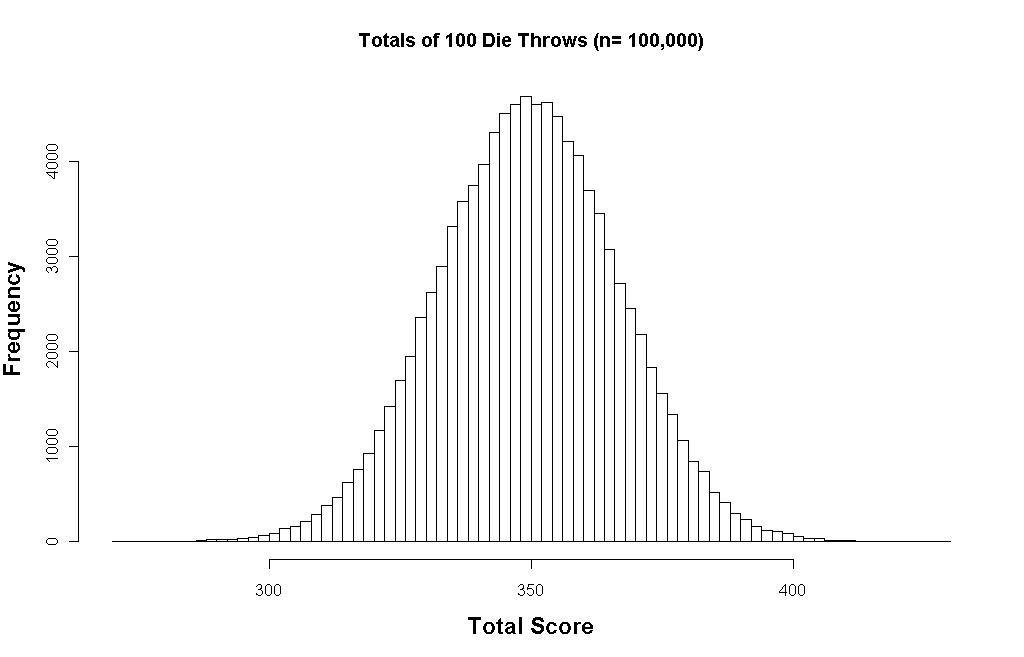
\includegraphics[scale=0.30]{images/3aDieHist3}
\end{center}

}

\frame{
\frametitle{Normal Distribution: Simulation Study}
Recall some observations made about the results of the simulation study, made in a previous lecture.
\begin{itemize}
% \item Approximately 76\% of the values are between 330 and 370.
\item Approximately 68.7\% of the values in the simulation study are between 332 and 367.
\item Approximately 95\% of the values are between 316 and 383.
\item $2.5\%$ of the values output are less than 316.
\item $2.5\%$ of the values study output are greater than 383.
\item 175 values are greater than or equal to 400, whereas 198 values are less than or equal to 300.
\item Results such as these are unusual, but they are not impossible.
\end{itemize}
}
%---------------------------------------------------------------%
\frame{
\frametitle{Normal Distribution: Simulation Study}
\begin{itemize}
\item Suppose we can \textbf{\emph{approximate}} the summation of the die-throws using the normal distribution. \smallskip
\item The normal mean is necessarily $\mu = 350$. \smallskip
\item The normal standard deviation is approximately 17. (68\% of values between $350 \pm 17$).\smallskip
\item Using the normal distribution, lets estimate the proportion of values greater than 383.
\end{itemize}
}

%---------------------------------------------------------------%
\frame{
\frametitle{Normal Distribution: Simulation Study}

\begin{center}
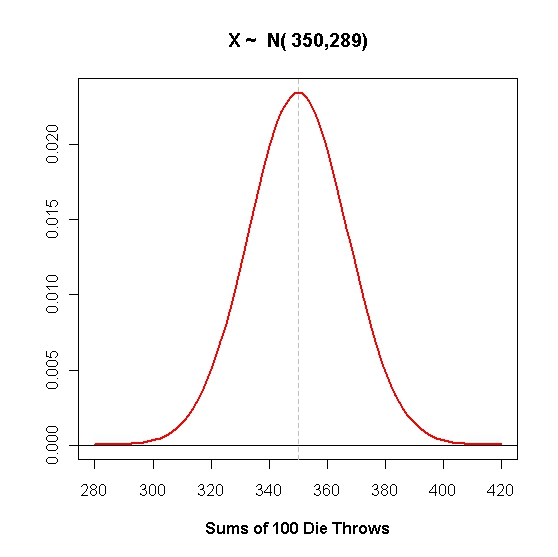
\includegraphics[scale=0.40]{images/5BNormalA}
\end{center}
}

%-------------------------------------------------------------%
\frame{
\frametitle{Normal Distribution: Simulation Study}
\begin{itemize}
\item X is the normal random variable that approximates the sum of values from 100 throws of a die.\smallskip
\item Find $P(X \leq 383)$\smallskip
\item First use the standardization formula to find the Z-score.
\[ z_o = {383 - 350 \over 17} = {33 \over 17} = 1.94 \]
\item Use the tables to compute $P(Z \geq 1.94)$ (\alert{Answer: 0.0262} )\smallskip
\item Because $P(Z \geq 1.94)  = 0.0262$, we can say $P(X \geq 383)  = 0.0262$
\item This is close to the proportion of observed values, which was 2.5\%.\smallskip
\item Remark : The standard deviation of 17 was an estimate. The actual standard deviation should 17.12.
\end{itemize}
}

\frame{
\frametitle{Normal Distribution: Simulation Study}

\begin{center}
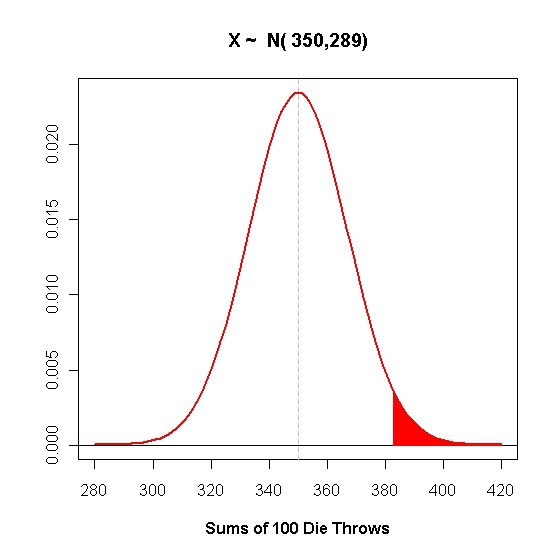
\includegraphics[scale=0.40]{images/5BNormalB}
\end{center}

}
%-------------------------------------------------------------%
\frame{
\frametitle{Working Backwards}
\begin{itemize}

\item Suppose we wish to find a value (lets call it A) from the normal distribution, such that a certain proportion of values is greater than A (e.g. 10\%)
\item Find A such that $P(X \geq A) = 0.10$. (with $\mu  = 350$ and $\sigma = 17$)
\item In general, our first step is to use the standardization equation to find the corresponding Z-score $z_A$.
\item Because we don't know what value A has, we can't use this approach.
\item However, we can say the following
\[  P(X \geq A) = P(Z \geq z_A) = 0.10 \]

\item From the tables, we can approximate a value for $z_A$, by finding the closest probability value, and determining the corresponding Z-score.
\end{itemize}
}

%------------------------------------------------------------------------%
\frame{

\frametitle{Find $z_A$ such that $ P(Z \geq z_a) = 0.10$}
\begin{itemize}
\item The closest probability value in the tables is $0.1003$.\\
\item The Z-score that corresponds to $0.1003$ is 1.28.\\
\item (Row : 1.2 , Column : 0.08)
\item Therefore $z_A  \approx 1.28$
\end{itemize}
\small
\begin{table}[ht]
%\caption{Standard Normal Distribution } % title of Table
\centering % used for centering table
\begin{tabular}{|c|| c c c c c c|} % centered columns (4 columns)
\hline %inserts double horizontal lines
& \ldots & \ldots & 0.006 &0.07&0.08&0.09 \\
%heading
\hline \hline% inserts single horizontal line
\ldots & \ldots & \ldots &\ldots& \ldots &\ldots&\dots \\ % inserting body of the table
1.0 & \ldots & \ldots &0.1446& 0.1423 &0.1401&0.1379 \\ % inserting body of the table
1.1 & \ldots & \ldots&0.1230& 0.1210 &0.1190&0.1170 \\ % inserting body of the table
1.2 & \ldots & \ldots&0.1038 & 0.1020 &\alert{0.1003}&0.0985\\
1.3 & \ldots & \ldots &0.0869& 0.0853 &0.0838&0.0823 \\ % inserting body of the table
\ldots & \ldots &\ldots&\ldots & \ldots &\ldots&\ldots\\
\hline %inserts single line
\end{tabular}
%\label{table:nonlin} % is used to refer this table in the text
\end{table}
}
%-------------------------------------------------------------%
\frame{
\frametitle{Working Backwards}
\begin{itemize}
\item We can now use the standardization formula.
\item We have only one unknown in the formula: $A$.
\[ 1.28 = {A - 350 \over 17} \]
\item Re-arranging ( multiply both sides by 17):\\
$ 21.76 = A - 350 $
\item Re-arranging ( add 350 to both sides ):\\
$ A = 371.76 $
\item $P(X \geq 371.76) \approx 0.10$
\item (Remark: for sums of die-throws, round it to nearest value)
\end{itemize}
}
%-----------------------------------------------------%
\end{document}
%-------------------------------------------------------------%
\frame{
\frametitle{Working Backwards: Another Example}
\begin{itemize}

\item Find B such that $P(X \geq B) = 0.90$. (with $\mu  = 350$ and $\sigma = 17$)
\item Necessarily $P(X \leq B) = 0.10$
\item Find some value $Z_B$ such that $P(Z \leq z_B) = 0.10$
\item $z_B$ could be negative.
\item Use the symmetry rule $P(Z \leq z_B) = P(Z \geq -z_B)$
\item $-z_B$ could be positive.
\item Based on last example $-z_B = 1.28$. Therefore $z_B = -1.28$
\end{itemize}
}
%-------------------------------------------------------------%
\frame{
\frametitle{Working Backwards}
\begin{itemize}
\item Again ,we can now use the standardization formula
\item We have only one unknown in the formula: $B$.
\[ -1.28 = {B - 350 \over 17} \]
\item Re-arranging ( multiply both sides by 17):\\
$ -21.76 = B - 350 $
\item Re-arranging ( add 350 to both sides ):\\
$ x_o = 350 - 21.76 = 328.24 $
\item $P(X \leq 328.24) \approx 0.10$
\end{itemize}
}
